
\section{Etapa 1: Definir Apariencia de la Aplicacion (Interfaz de usuario) }
%\section{Etapa 1: Definir Apariencia de la Aplicacion (Interfaz de usuario) }
\begin{frame}[fragile]
\frametitle{Fase 1: Dividir la pantalla en contenedores verticales} 
\begin{columns}
\column{0.78\linewidth}
\begin{block}{Archivo \textbf{activity\_main.xml}}
%\input{Layout_Fase1.xml}
\inputminted[highlightlines={7-11},linenos,fontsize=\tiny]{xml}{00_CambiosInterfaz/Layout_Fase1.xml}

\end{block}
\column{0.20\linewidth}
%\begin{block}{Archivo \textbf{MainActivity.kt}}
%\begin{minted}[linenos,fontsize=\tiny]{kotlin}
%\end{minted}
%\end{block}
\begin{center}
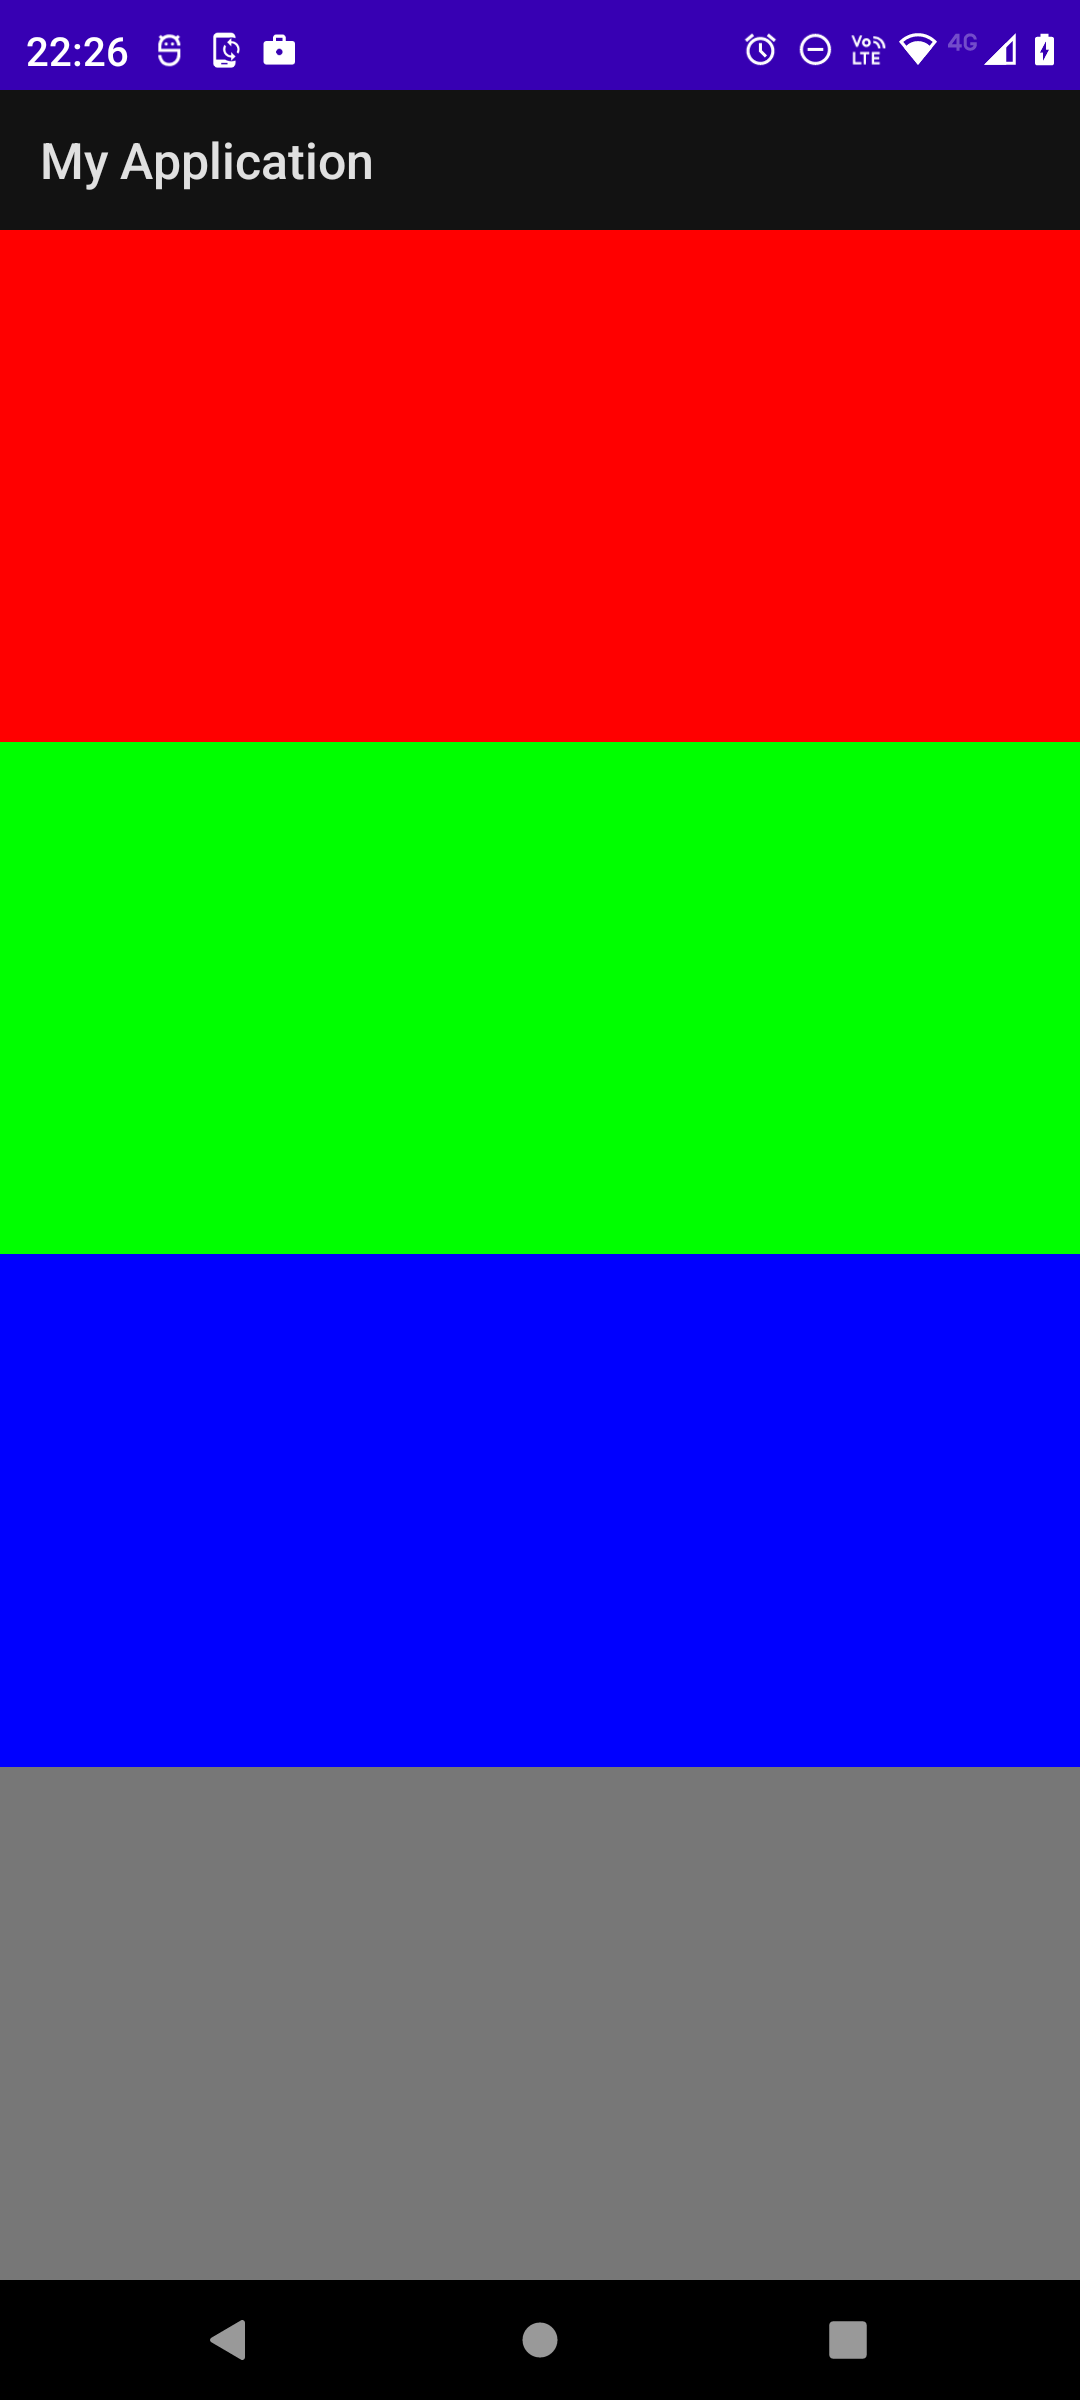
\includegraphics[width=0.95\linewidth]{00_CambiosInterfaz/Fase1.png}    
\end{center}
\end{columns}
\end{frame}


\begin{frame}[fragile]
\frametitle{Fase 2: Agregar un contenedor horizontal dentro de uno vertical} 
%Sustituir solo las lineas 7-10 del layout anterior con el archivo mostrado
Este fragmento de c\'odigo sustituye a las lineas 7 a 10 del \textit{activity\_main.xml}
\begin{columns}
\column{0.78\linewidth}
\begin{block}{Porci\'on del Layout que incluye tres contenedores verticales}
\inputminted[linenos,fontsize=\tiny]{xml}{00_CambiosInterfaz/Layout_Fase2.xml}
\end{block}
\column{0.20\linewidth}
%\begin{block}{Archivo \textbf{MainActivity.kt}}
%\begin{minted}[linenos,fontsize=\tiny]{kotlin}
%
%\end{minted}
%\end{block}
\begin{center}
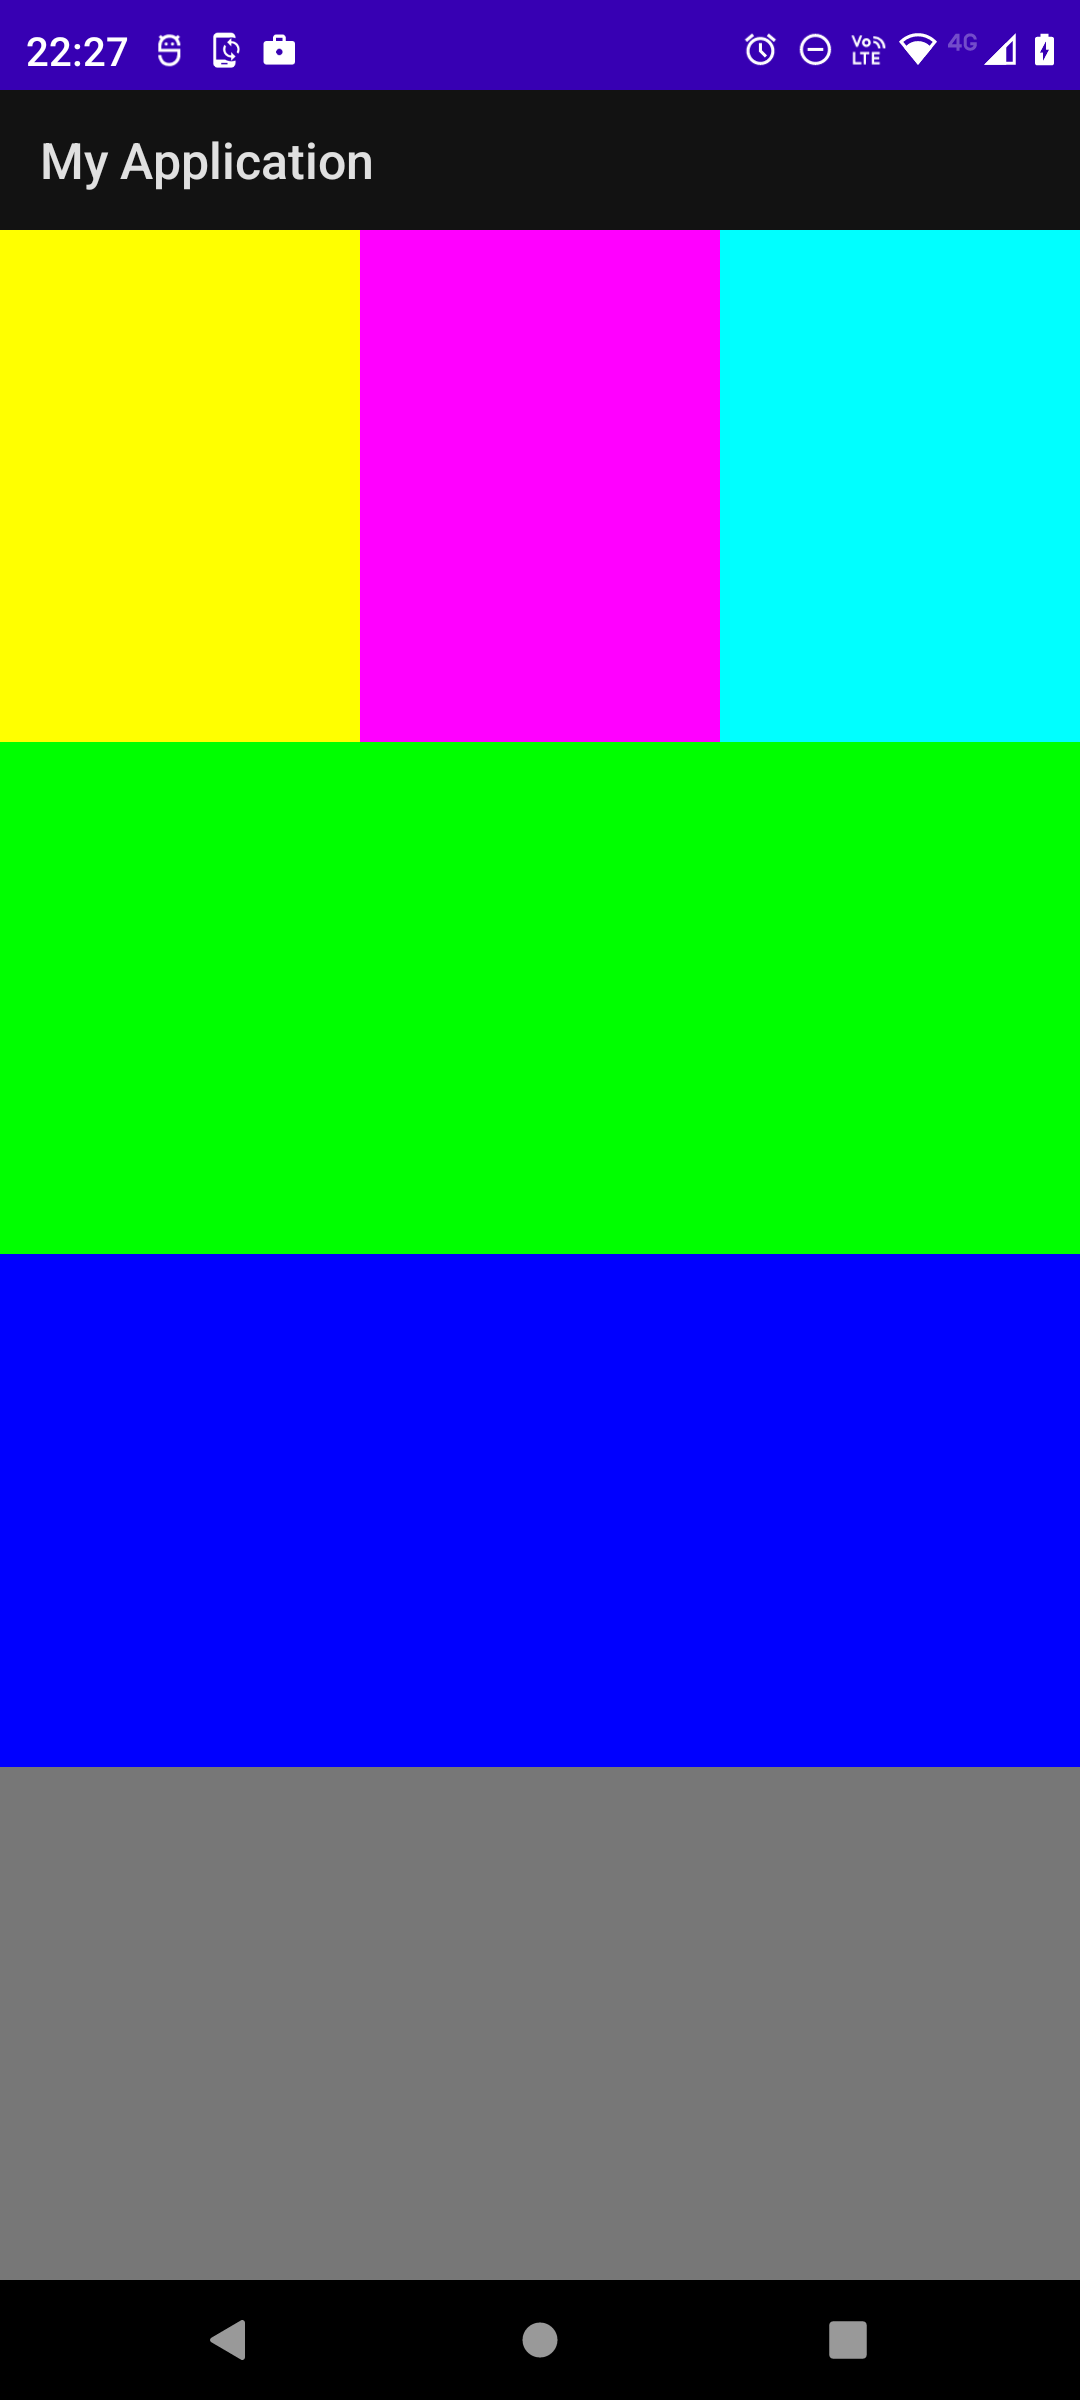
\includegraphics[width=0.95\linewidth]{00_CambiosInterfaz/Fase2.png}    
\end{center}
\end{columns}
\end{frame}

\begin{frame}[fragile]
\frametitle{Aplicaci\'on TIC-TAC-TOE} 
\begin{columns}
\column{0.50\linewidth}
\begin{itemize}
\item Juego para dos jugadores
\item Cada jugador juega una de dos posibles combinaciones (circulo o tacha)
\item El control debe decidir cuando un jugador gana o cuando hay empate
\item Llevar el manejo de los turnos
\item Requerimos un componente de interfaz que se comporte como un boton y que despliegue una imagen. Soluci\'on: \textit{ImageButton}
\end{itemize}
\column{0.50\linewidth}
\begin{center}
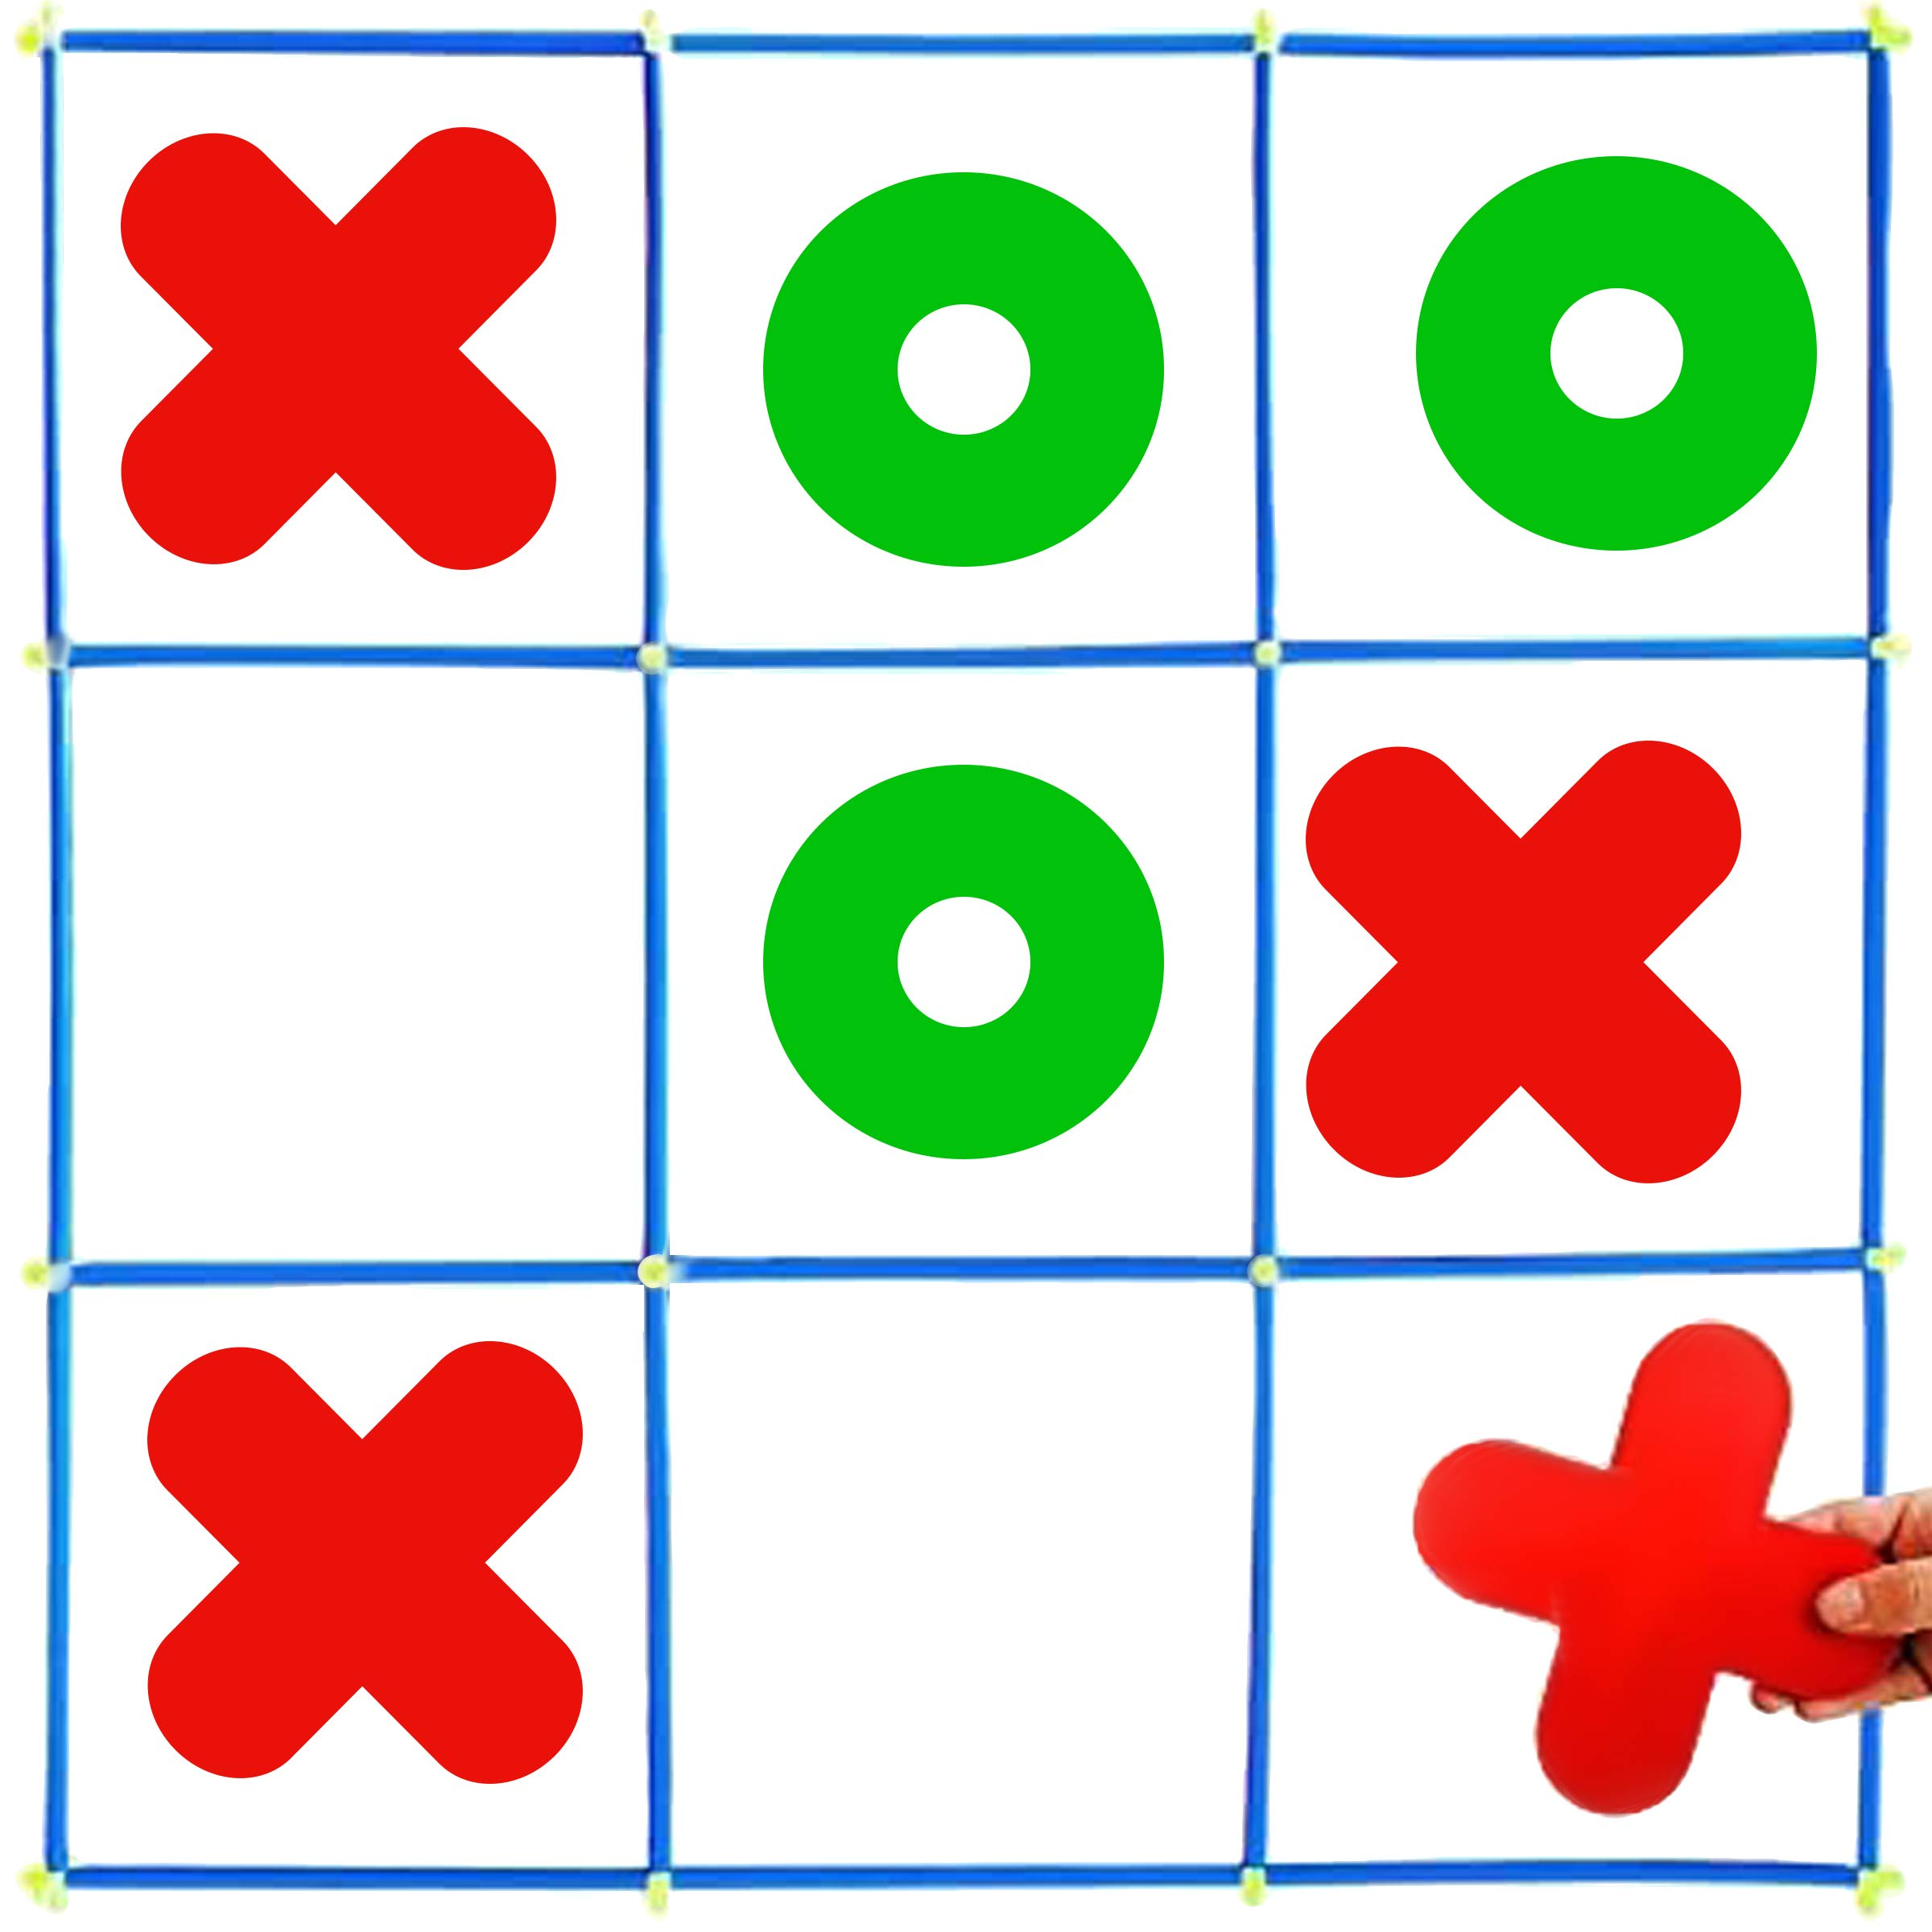
\includegraphics[width=0.95\linewidth]{00_CambiosInterfaz/TicTacToe.jpg}    
\end{center}

\end{columns}
\end{frame}


\begin{frame}[fragile]
\frametitle{Fase 3 (Parte 0): Agregar Imagenes que seran utilizadas como iconos} 
\begin{itemize}
\item Localizar la carpeta \textit{drawable} dentro de la carpeta \textit{res}
\item De la carpeta Github, descargar las imagenes usuario.png, cruz.png y corazon.png y copiar estas imagenes en la carpeta antes mencionada
\end{itemize}
\begin{center}
\begin{tabular}{ccc}
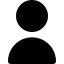
\includegraphics[width=0.32\linewidth]{00_CambiosInterfaz/usuario.png}  &

\includegraphics[width=0.32\linewidth]{00_CambiosInterfaz/cruz.png}  &

\includegraphics[width=0.32\linewidth]{00_CambiosInterfaz/corazon.png}   
\end{tabular}
\end{center}
\end{frame}


\begin{frame}[fragile]
\frametitle{Fase 3 (Parte 1): Agregar 3 botones en orientaci\'on al contenedor horizontal al primer Contenedor} 
\begin{columns}

\column{0.78\linewidth}
%Sustituir solo las lineas 7-10 del layout anterior con el archivo mostrado
Este fragmento de c\'odigo sustituye a las lineas 7 a 10 del \textit{activity\_main.xml}
\begin{block}{Primer Layout Horizontal incluido tres \textit{ImageButtons}}
\inputminted[linenos,fontsize=\tiny]{xml}{00_CambiosInterfaz/Layout_Fase3.xml}
\end{block}
\column{0.2\linewidth}
%\begin{block}{Archivo \textbf{MainActivity.kt}}
%\begin{minted}[linenos,fontsize=\tiny]{kotlin}
%
%\end{minted}
%\end{block}
\begin{center}
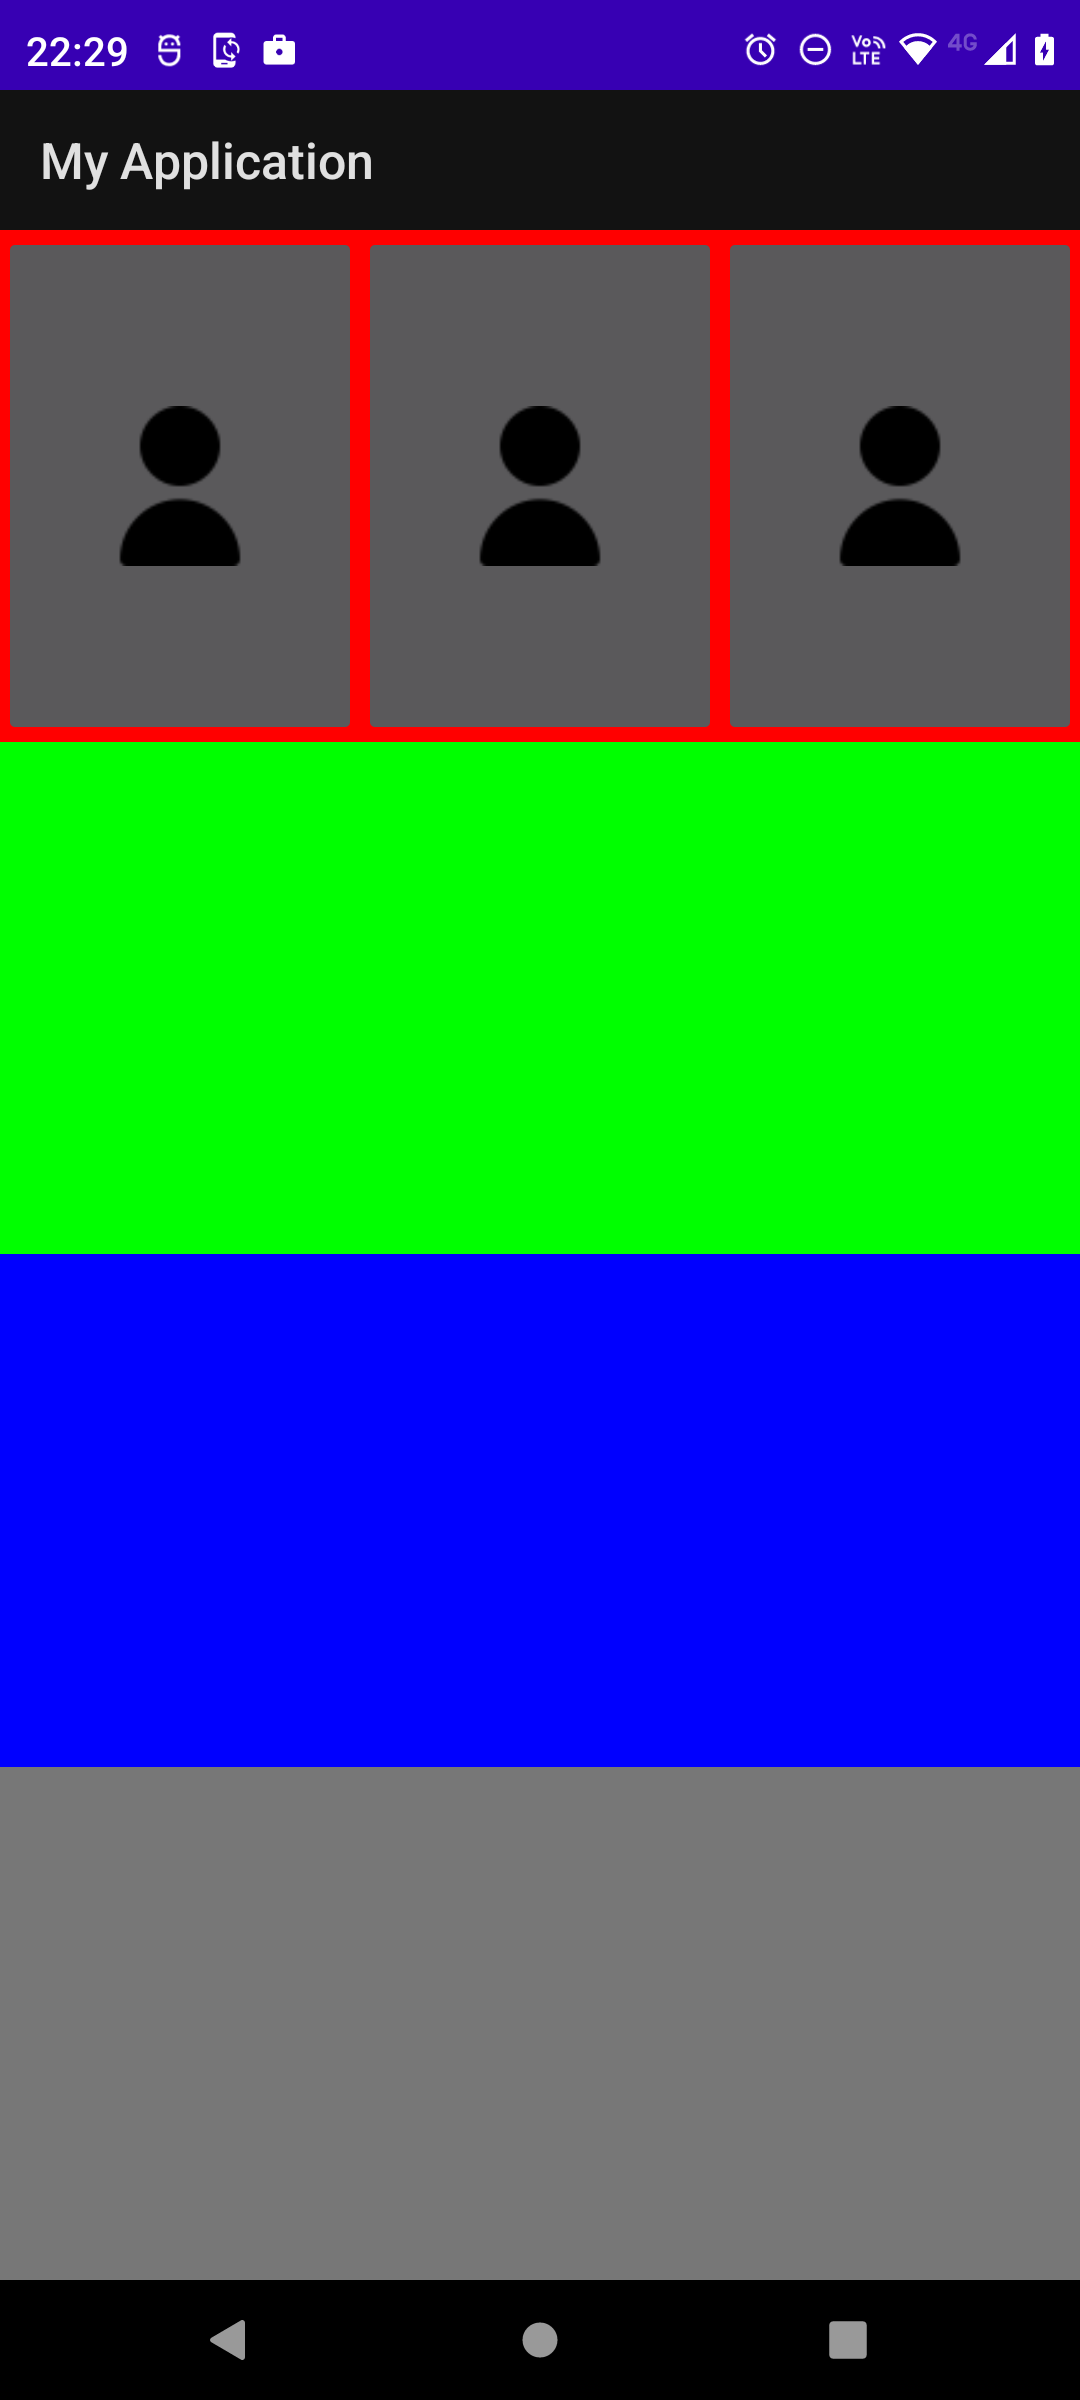
\includegraphics[width=0.95\linewidth]{CapturasPantalla/Fase3.png}    
\end{center}
\end{columns}
\end{frame}

\begin{frame}[fragile]
\frametitle{Fase 3 (Parte 2): Repetir para los otros contenedores} 
\begin{columns}
\column{0.98\linewidth}
Este fragmento de c\'odigo sustituye a las lineas 12 a 21 del \textit{activity\_main.xml}
\begin{block}{Segundo y tercer Layouts horizontales, cada uno con tres \textit{ImageButtons}}
\inputminted[linenos,fontsize=\tiny]{xml}{00_CambiosInterfaz/Layout_Fase3B.xml}
\end{block}
\column{0.02\linewidth}
\begin{center}
%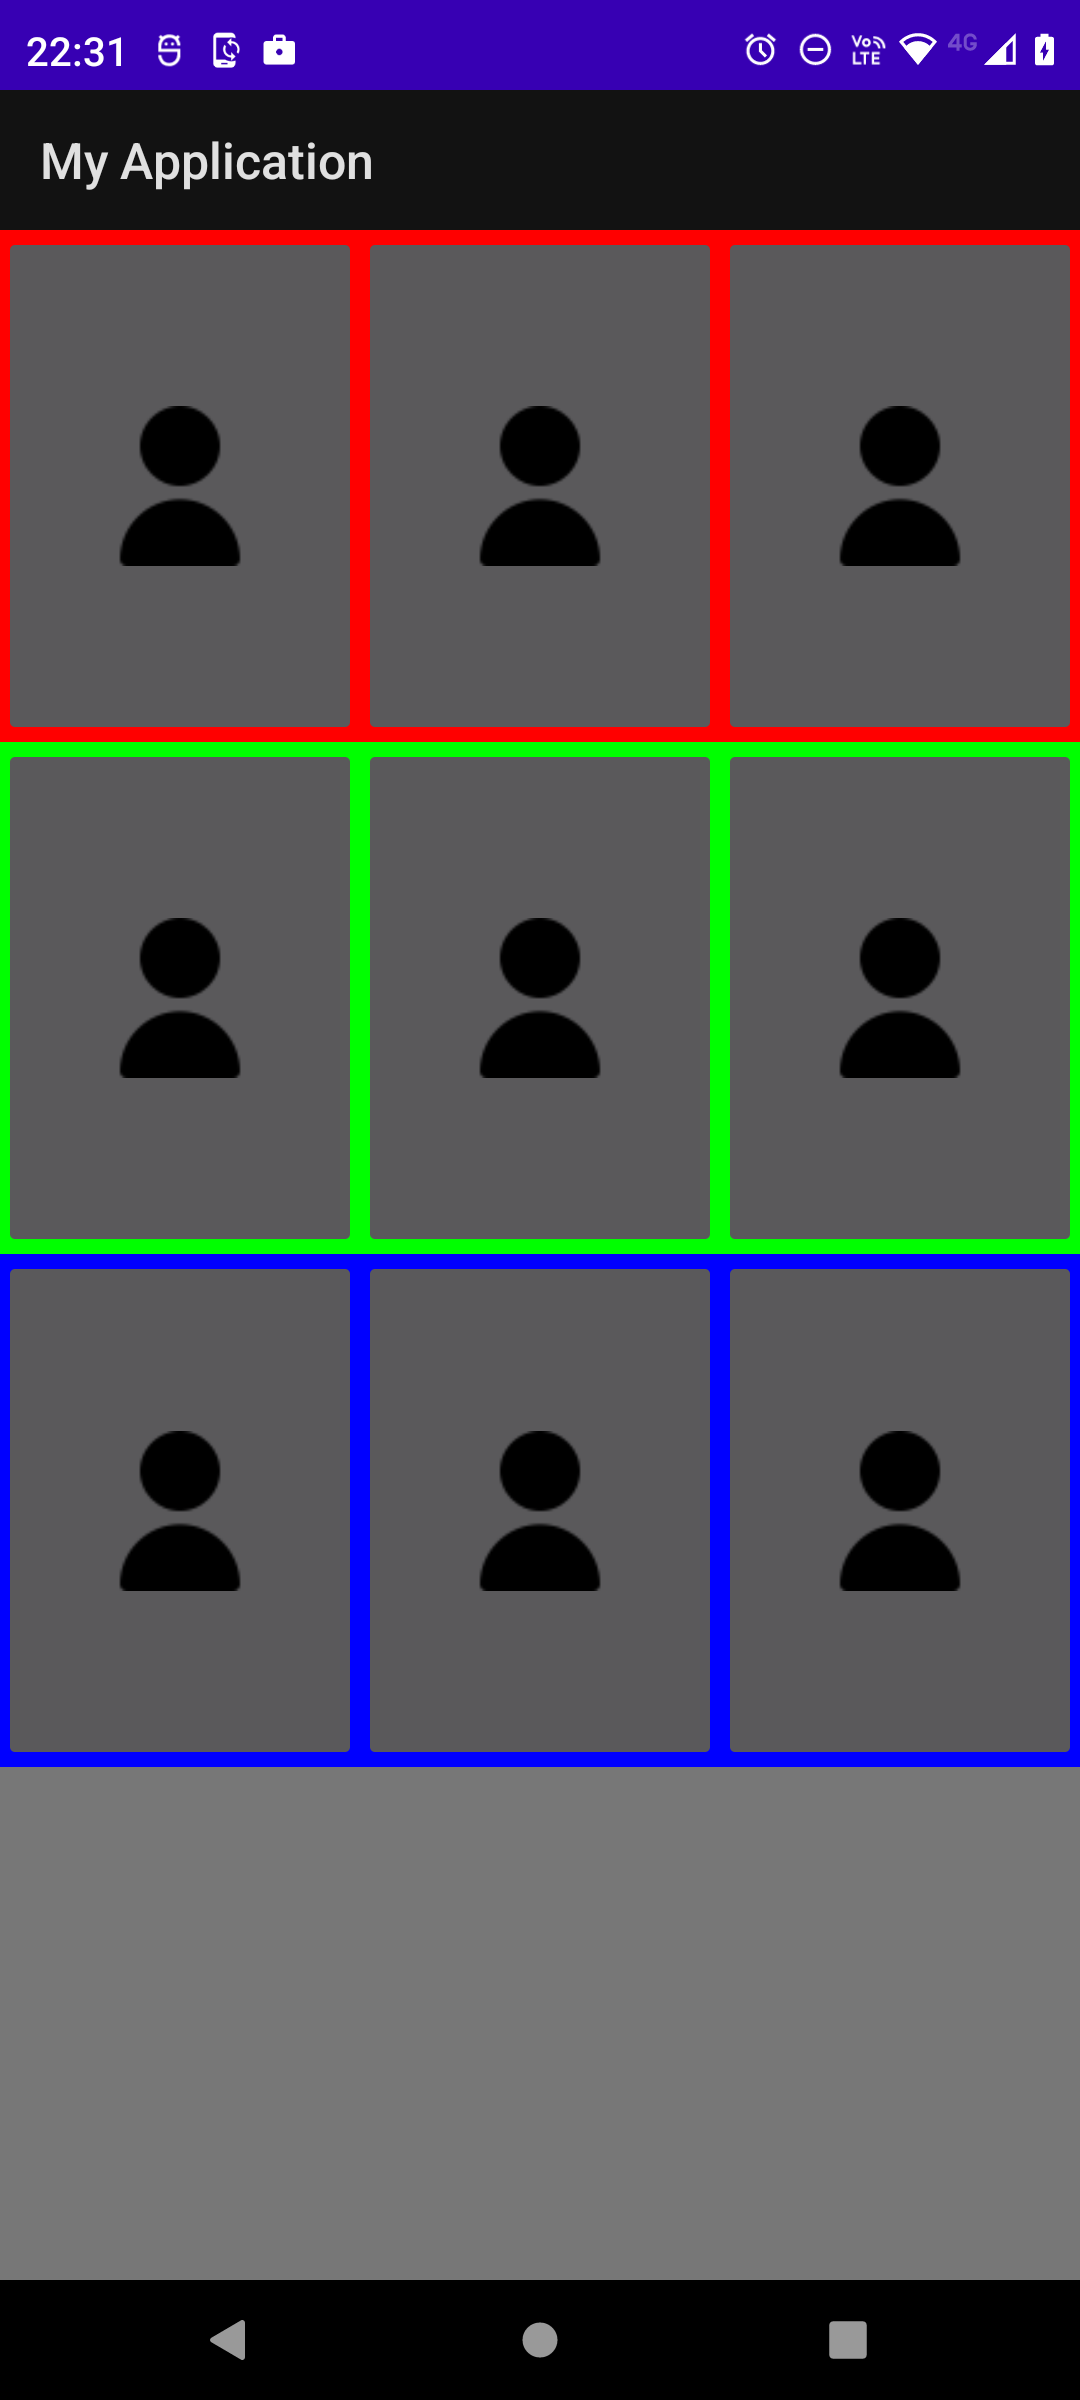
\includegraphics[width=0.95\linewidth]{CapturasPantalla/Fase3C.png}    
\end{center}
\end{columns}
\end{frame}



\begin{frame}[fragile]
\frametitle{Fase 3 (Parte 3): Al ultimo contenedor agregar un TextView} 
\begin{columns}

\column{0.70\linewidth}
Este fragmento de c\'odigo sustituye a las lineas 22 a 26 del \textit{activity\_main.xml}
\begin{block}{\'Ultimo contenedor del Layout}
\inputminted[linenos,fontsize=\tiny]{xml}{00_CambiosInterfaz/Layout_Fase3C.xml}
\end{block}
\column{0.20\linewidth}
\begin{center}
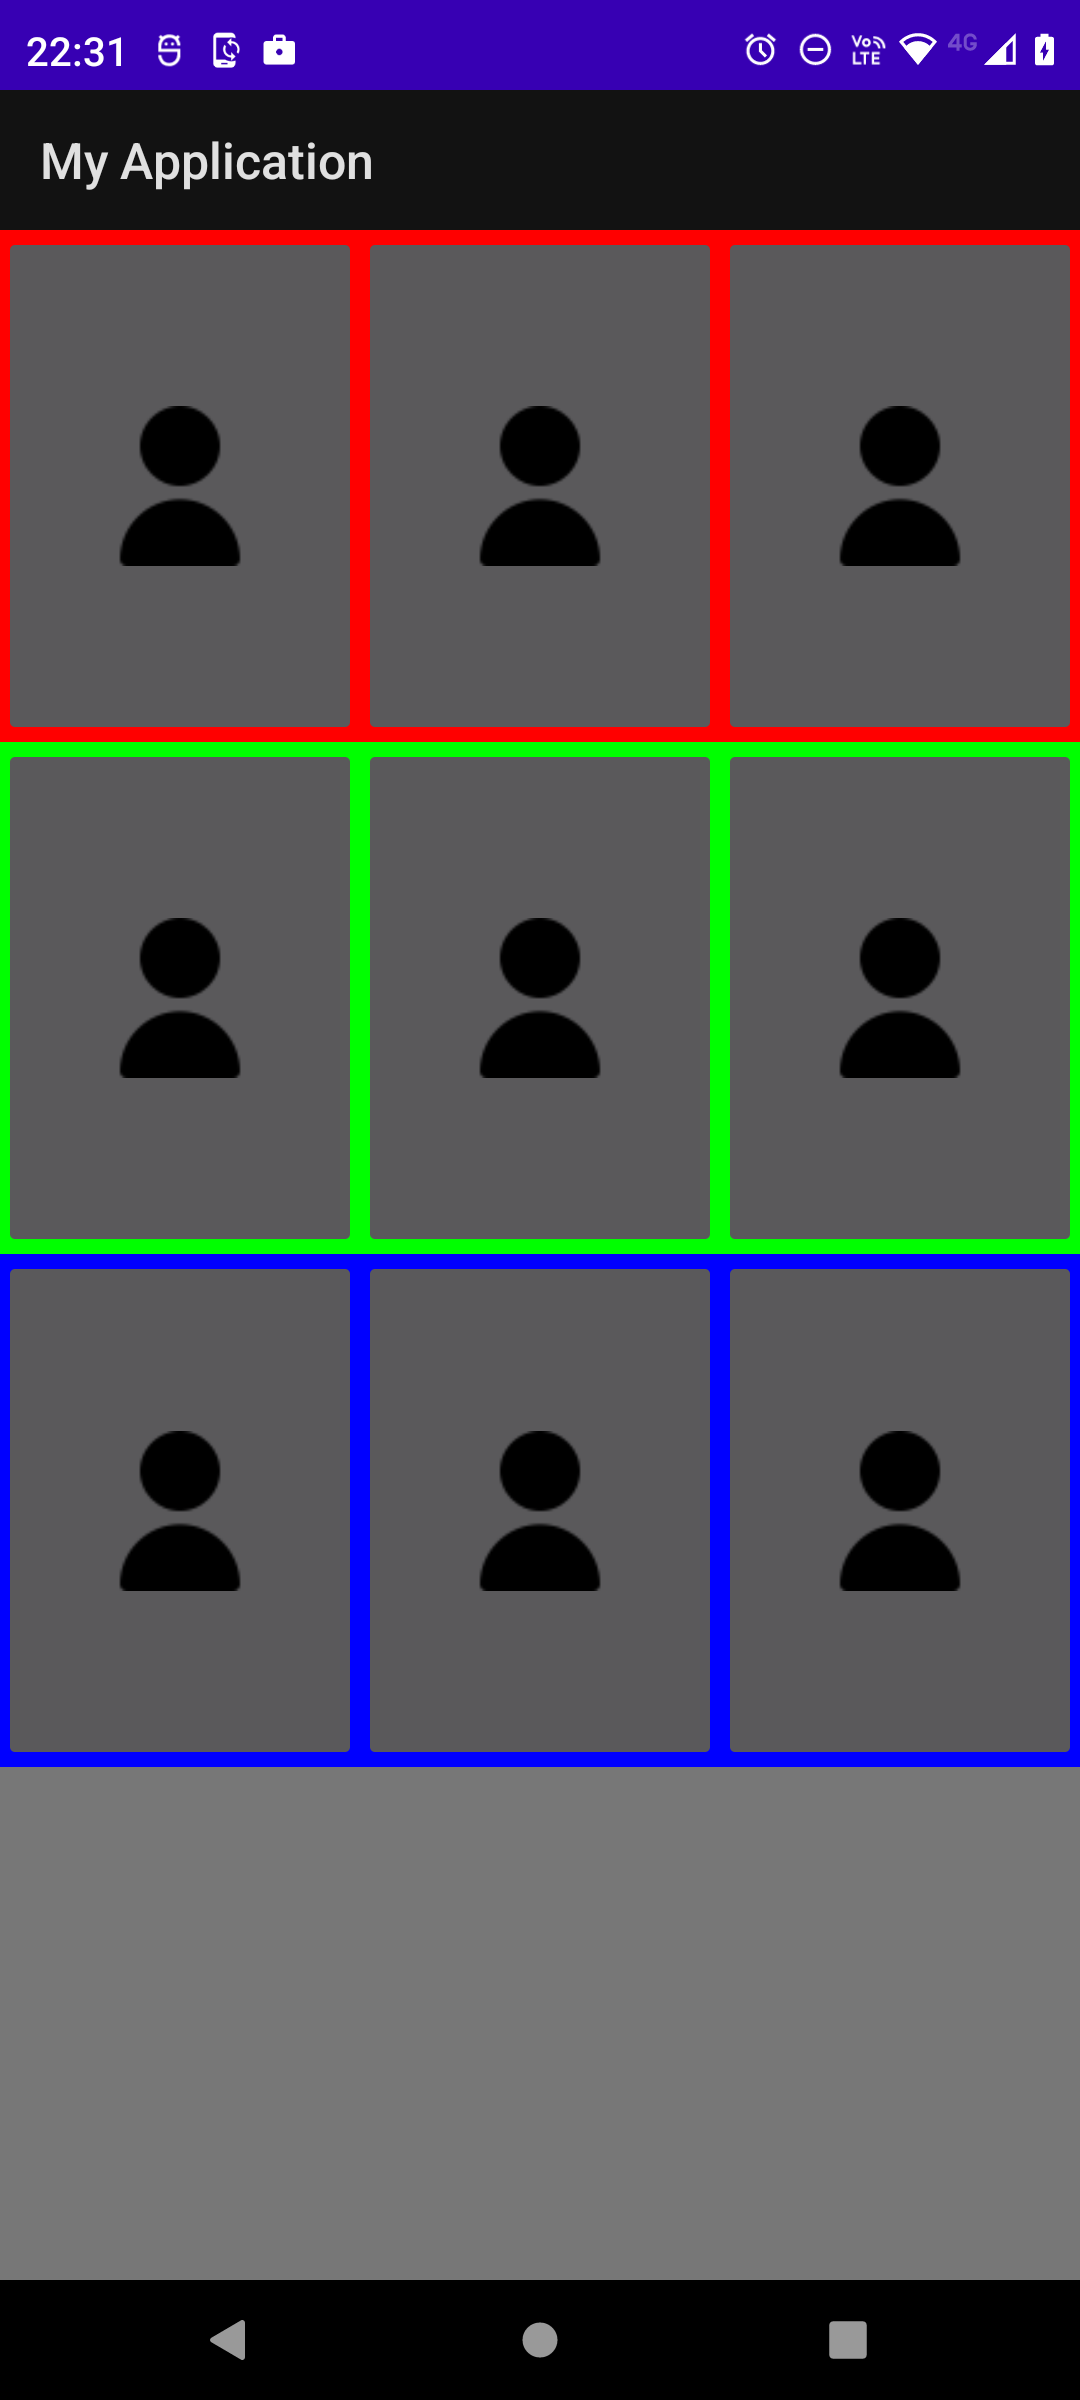
\includegraphics[width=0.95\linewidth]{CapturasPantalla/Fase3C.png}    
\end{center}
\end{columns}
\end{frame}

\begin{frame}[fragile]
\frametitle{Codigo Completo} 
\begin{columns}
\column{0.950\linewidth}
\begin{block}{P1}
\begin{minted}[linenos,fontsize=\tiny]{xml}
<?xml version="1.0" encoding="utf-8"?>
<LinearLayout xmlns:android="http://schemas.android.com/apk/res/android"
    xmlns:app="http://schemas.android.com/apk/res-auto"
    xmlns:tools="http://schemas.android.com/tools"
    android:layout_width="match_parent" android:layout_height="match_parent"
    android:orientation="vertical" tools:context=".MainActivity">
    <LinearLayout android:background="#ff0000"
        android:layout_width="match_parent"
        android:layout_height="0dp"
        android:layout_weight="1">
        <ImageButton android:id="@+id/boton1_1"
            android:src="@drawable/usuario"
            android:layout_width="0dp"
            android:layout_height="match_parent"
            android:layout_weight="1"/>
        <ImageButton android:id="@+id/boton1_2"
            android:src="@drawable/usuario"
            android:layout_width="0dp"
            android:layout_height="match_parent"
            android:layout_weight="1"/>
        <ImageButton android:id="@+id/boton1_3"
            android:src="@drawable/usuario"
            android:layout_width="0dp"
            android:layout_height="match_parent"
            android:layout_weight="1"/>
    </LinearLayout>
\end{minted}
\end{block}
\end{columns}
\end{frame}

\begin{frame}[fragile]
\frametitle{Codigo Completo (2)} 
\begin{columns}
\column{0.950\linewidth}

\begin{block}{P2}
\begin{minted}[linenos,fontsize=\tiny]{xml}
    <LinearLayout android:background="#00ff00" android:layout_width="match_parent"
        android:layout_height="0dp" android:layout_weight="1">
        <ImageButton android:id="@+id/boton2_1"
            android:src="@drawable/usuario" android:layout_width="0dp"
            android:layout_height="match_parent" android:layout_weight="1"/>
        <ImageButton android:id="@+id/boton2_2"
            android:src="@drawable/usuario" android:layout_width="0dp"
            android:layout_height="match_parent" android:layout_weight="1"/>
        <ImageButton android:id="@+id/boton2_3"
            android:src="@drawable/usuario" android:layout_width="0dp"
            android:layout_height="match_parent" android:layout_weight="1"/>
    </LinearLayout>
    <LinearLayout android:background="#0000ff" android:layout_width="match_parent"
        android:layout_height="0dp" android:layout_weight="1">
        <ImageButton android:id="@+id/boton3_1"
            android:src="@drawable/usuario" android:layout_width="0dp"
            android:layout_height="match_parent" android:layout_weight="1"/>
        <ImageButton android:id="@+id/boton3_2"
            android:src="@drawable/usuario" android:layout_width="0dp"
            android:layout_height="match_parent" android:layout_weight="1"/>
        <ImageButton android:id="@+id/boton3_3"
            android:src="@drawable/usuario" android:layout_width="0dp"
            android:layout_height="match_parent" android:layout_weight="1"/>
    </LinearLayout>
\end{minted}
\end{block}
\end{columns}
\end{frame}


\begin{frame}[fragile]
\frametitle{Codigo Completo} 
\begin{columns}
\column{0.950\linewidth}
\begin{block}{P3}
\begin{minted}[linenos,fontsize=\tiny]{xml}

    <LinearLayout android:background="#777777"
        android:layout_width="match_parent"
        android:layout_height="0dp"
        android:layout_weight="1">
        <TextView android:id="@+id/textView_Pizarra_Estatus"
            android:layout_width="match_parent"
            android:layout_height="match_parent"
            android:textSize="18dp"
            android:gravity="center"/>
    </LinearLayout>
</LinearLayout>
\end{minted}
\end{block}
\end{columns}
\end{frame}





